\usepackage[authoryear,round]{natbib}
\usepackage{multirow}

\newcommand{\sheetnum}{%
	07
}
%\setcounter{section}{\sheetnum-3}
\newcommand{\tutorialtitle}{%
    Stochastic Optimization
}
\newcommand{\tutorialtitleshort}{%
	Stochastic Optimization
}
% for slides
\subtitle{\sheetnum \tutorialtitle}

\maxdeadcycles=1000 % Workaround for ! Output loop---100 consecutive dead cycles because of too many figures

% The following use of algroithms is recommended for the notes:
%
%\begin{figure}[!t]
%\removelatexerror
%\begin{algorithm}[H]
    % your algo here
    %\label{alg:algolabel}
    %\caption{algocaption}
%\end{algorithm}
%\end{figure}
%\begin{algorithm}
% Below is the definition for the command \removelatexerror:
\makeatletter
\newcommand{\removelatexerror}{\let\@latex@error\@gobble}
\makeatother

\begin{document} %%%%%%%%%%%%%%%%%%%%%%%%%%%%%%%%%%%%%%%%%%%%%%%%%%%%%%%

\sheet{\sheetnum}{\tutorialtitleshort}

\ttopic{\tutorialtitle}

\begin{frame}
\titlepage
\end{frame}

\begin{frame}
\mode<presentation>{
\tableofcontents[hideallsubsections]
}
\mode<article>{
\tableofcontents
}
\end{frame}

\newpage

% The variable mycolumnleft is set in the minotes class
% The column settings are ignored by the slides
\columnratio{\mycolumnleft,1-\mycolumnleft}
\begin{paracol}{2}
%\setlength{\columnseprule}{0.1pt}
%\setlength{\columnsep}{5em}

\begin{rightcolumn}

\mode<all>
\section{Limitations in how we've been optimizing so far}

\begin{frame}

Our iterative gradient-based optimizations:
\begin{itemize}
\item assumes the optimum ``up ahead'' is the best solution,

\begin{figure}[ht]
  \centering
  \begin{tabular}{c c}
      \includegraphics[height=3.5cm]{img/gradient-descent.pdf} &
      \includegraphics[height=3.5cm]{img/gradient-descent_local.pdf}
  \end{tabular}
  \notesonly{
  \caption{Learning by gradient descent}\label{fig:graddescent}
  }
\end{figure}

\item doesn't handle discrete optimization.
\end{itemize}

\end{frame}

\mode*

\mode<all>
\section{Exploration vs. Exploitation}

\notesonly{
%An
%introduction illustrating the underlying analogy can be found in
%\textcite[ch. 7]{DudaEtAl2001}.  \textcite{Murphy2012} gives a good
%and extensive discussion of undirected graphical models (Markov Random
%fields, ch~19), variational inference (ch~21; mean field for the ISING
%model, ch~21.3), and Monte Carlo Methods (ch~23), as well as MCMC
%methods (ch~24). Further information regarding variational methods can
%be found in \textcite{Bishop2006}.

Learning is about tuning model parameters to fit some objective given training data. 
For simple models with only few parameters one can formulate an analytic solution that optimizes the objective and yields the optimal parameters directly. 
As soon as the number of parameters increases, we opt for iterative gradient-based methods for finding the extrema of the objective function. If we were trying to minimize some cost function $E$, 
iteratively updating the parameters $\vec w$ by moving them in the direction of where the gradient points steepest leads to the location of an extremum. 
However, the cost function may contain multiple extrema, and there is no guarantee gradient-based learning will take us to a \emph{global} or \emph{local} optimum. 
Following the gradient assuming that it will lead to a solution that represents the global optimum is considered a \emph{greedy} approach to learning. 

Completely abandoning such assumptions will lead to a \emph{random search} for the optimal parameters. When the previous set of parameters has no influence on the choice of weights in the next iteration, 
then our learning approach is dominated by \emph{exploration} as opposed to \emph{exploitation} when we learn in a greedy fashion.
}

\begin{frame}{Exploration vs. Exploitation}

\begin{figure}[ht]
  %\centering
  \begin{tabular}{c c}
	  \visible<2->{exploration} & exploitation\\
      \visible<2->{\includegraphics[height=3.0cm]{img/exploration.pdf}} &
      \includegraphics[height=3.0cm]{img/exploitation.pdf} \\
      \visible<2->{random search} & greedy search/hill ``climbing''
      \end{tabular}
  \notesonly{
  \caption{exploration vs. exploitation}
  }
  \label{fig:exploration-exploitation}
\end{figure}

\pause

\question{What are the advantages and disadvantages of exploration?}

\notesonly{
The advantage of exploration is that we always discard a set of parameters if the next set yields a better cost value. Therefore, exploration is not prone to getting stuck inside a local optimum. The obvious disadvantage is that there are no guarantees on how long it will take to find the global optimum. We never know if we've converged or not. Exploitation, or the greedy approach (with the appropriate learning rate schedule) is able to converge. However, whether it reaches a global or local solution depends on the starting position.
}


\end{frame}

%\underline{Motivation 1:} We will look at how stochastic optimization can find a tradeoff between the two modes exploration and exploitation.

\mode*

\mode<all>
\section{Discrete Optimization}

\begin{frame}

\slidesonly{
\begin{block}{Supervised \& unsupervised learning $\rightarrow$ evaluation of cost function $E$}
Find the arguments that optimize $E$.
\begin{itemize}
 \item real-valued arguments: gradient based techniques (e.g. ICA unmixing matrices)
 \item discrete arguments: ??? (e.g. for cluster assignment)
\end{itemize}
\end{block}
}
\notesonly{
So far we've been concerned with optimization problems with real valued arguments. The free parameters form a continuous space. The direction of the principle components in PCA and the unmixing matrix we are trying to find in ICA are real-valued arguments to their respective problems.
Gradient-based solutions are well suited for real-valued arguments as we tune the weights to minimize to optimize the cost function.

But what if the problem we are trying to optimize operate on discrete arguments. This could be the case if we were tackling a problem such as K-Means clustering. K-Means clustering involves finding arguments with which to assign an observation to one of multiple clusters. The cost function that measures the quality of the assignments is continuous but the arguments we optimize over, which effectively assign each observation to one cluster instead of another cluster, are discrete variables. Below is an example of such an assignment:


}

\only<1>{

\begin{figure}[ht]
  \centering
  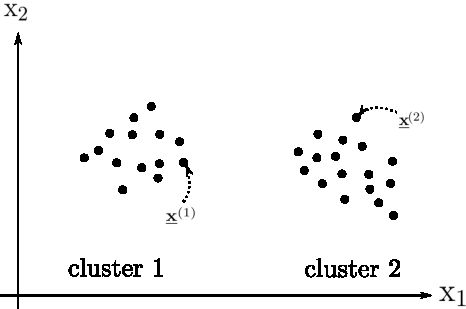
\includegraphics[height=3.5cm]{img/clustering.pdf}
  \caption{Clustering involves discrete-valued arguments.}
  \label{fig:clustering}
\end{figure}
}

\only<2>{

\begin{center}
  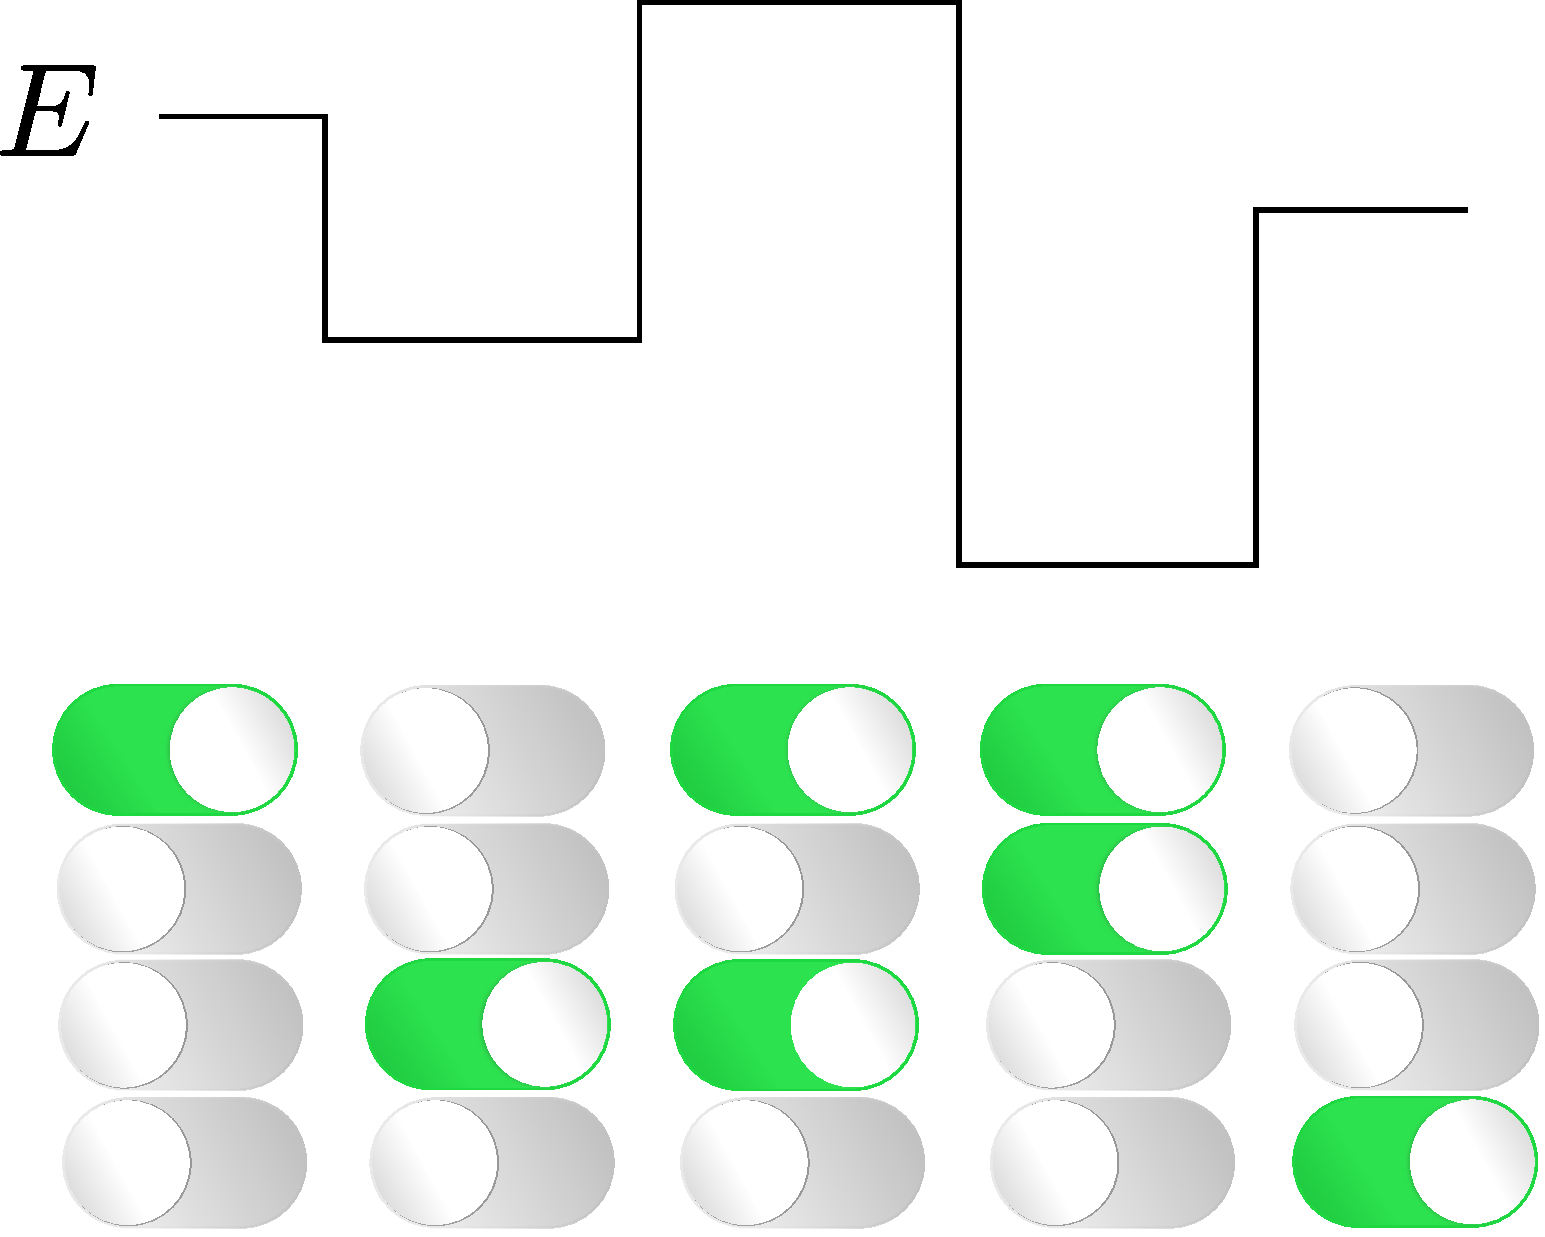
\includegraphics[height=3.5cm]{img/cyberscooty-switch_1-5}
  \notesonly{\captionof{figure}{A combinatorial problem}}
\end{center}
}


\end{frame}

%\newpage

\subsection{Formalization of the discrete optimization problem}

\begin{frame}{\subsecname}

\begin{block}{Setting} 
\begin{itemize}
 \item discrete variables $s_i, \ i = 1, \ldots, N\quad$ (e.g. $s_i \in \{+1, -1\}$  \notesonly{``binary units''} or $s_i \in \mathbb N$) 
 % $s_i \in \{1, 2, \dots 9 \} $ 
 \item \indent short-hand notation: $\vec{s}$ (``state'') -- { $\{\vec{s}\}$ is called state space }
 \item {cost function:} $E: \vec{s} \mapsto E_{(\vec{s})} \in \mathbb{R}$ -- { not restricted to learning problems}
\end{itemize}
\end{block}

We will focus on \textbf{minimization} problems.

\begin{block}{Goal: find state $\vec{s}^*$, such that:} 
\begin{equation*}
	E \eqexcl \min \qquad (\text{desirable global minimum for the cost})
\end{equation*}
Consequently,
\begin{equation*}
	s^* := \argmin E.
\end{equation*}
\end{block}
\end{frame}

\subsubsection{Strategies for discrete optimization}

\begin{frame}{\subsubsecname}

\notesonly{
We want to find the best configuration of a discrete system (e.g.\
state of interacting binary units). Evaluating full search space works only for
very small problems ($\rightarrow 2^N$ possibilities for a problem with $N$
binary units, search space is the set of corners of a
hypercube). A greedy strategy will often get trapped if there are
multiple local minima.
}

\begin{itemize}
\item Evolutionary and genetic algorithms (GA) have been
  motivated by \emph{biological} phenomena of adaptation through
  \emph{mutation} and \emph{selection}.

\vspace{5mm}
  
\item GA and Monte-Carlo-Markov-Chain methods based on a \emph{proposal} and
  \emph{acceptance} strategy ($\rightarrow$ Metropolis) can be interpreted
  as ``learning via trial and error''. \emph{Simulated annealing} falls within MCMC.
\end{itemize}
\end{frame}


\mode*

\clearpage

\mode<all>
\section{Simulated (stochastic) annealing}

\mode<presentation>{
\begin{frame} 
    \begin{center} \huge
        \secname
    \end{center}
	%\begin{center}
	%Dealing with the diverging hebbian rule\\
	%through implicit normalization
	
	%\end{center}
    \begin{center}
		
\includegraphics[width=3cm]{img/380px-Blacksmith_anvil_hammer}
    \end{center}
\end{frame}
}

\begin{frame}{\secname}

\emph{Simulated annealing}\notesonly{\footnote{
The ``annealing'' part in the name comes from metallurgy. As metals cool down, the movement of the atoms slows down and their kinetic energy decreases until the metal eventually hardens.
}}
\notesonly{is a method for stochastic optimization with which we can find a tradeoff between exploitation and exploration. More importantly, it is designed to cope with optimization of discrete-valued arguments. Simulated annealing is
  motivated by phenomena in physics related to the organization and
  alignment of microscopic components forming specific macroscopic
  configurations. }
\slidesonly{\\$\leadsto$ exploitation and exploration tradeoff}
\slidesonly{\\$\leadsto$ (more importantly) discrete optimization\\\vspace{0.5cm}}

\end{frame}

\begin{frame}{\secname}

\svspace{-5mm}

\question{What does simulated annealing do?}

- In the case of \emph{minimization} it:

\begin{enumerate}
\item describes a strategy for switching between states
\item increases the probability of landing in lower-energy states\footnote{This preference for lower-energy states is specific to \emph{minimization} problems.}
\item allows for escaping \textbf{local} optima
\end{enumerate}


\begin{center}
	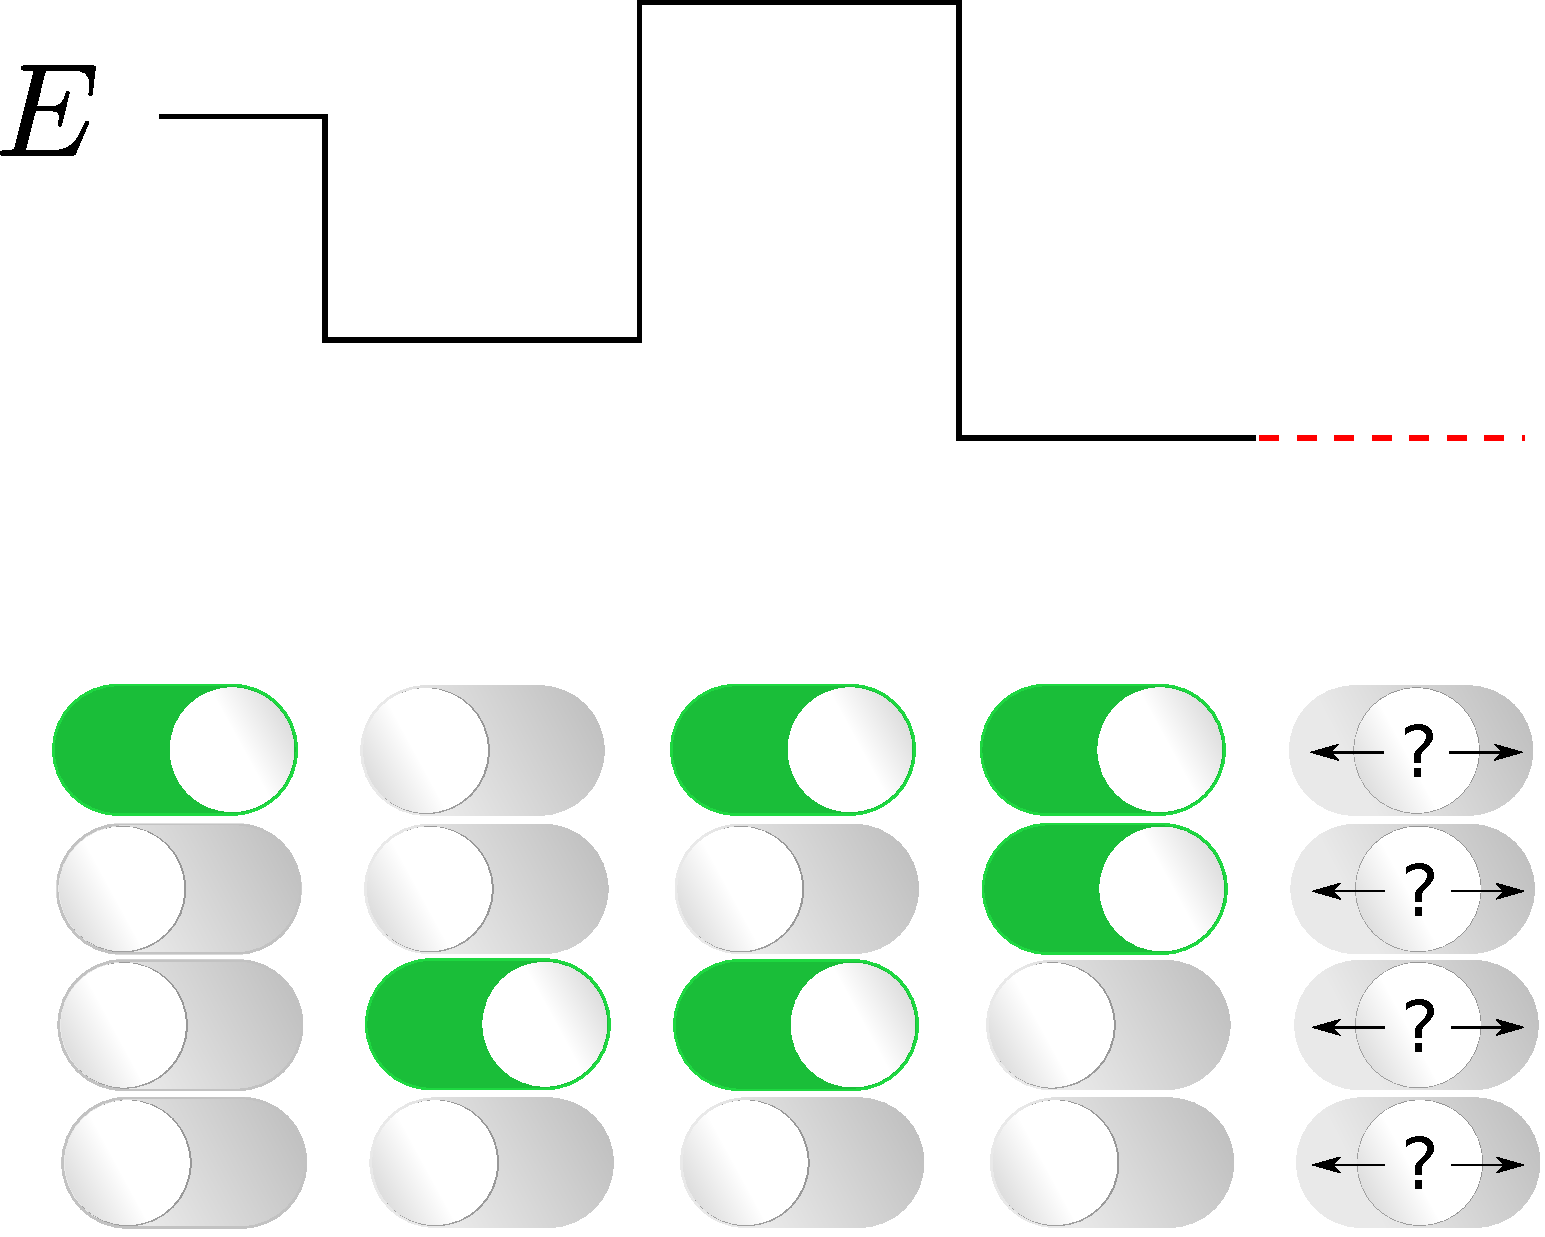
\includegraphics[width=5cm]{img/cyberscooty-switch_1-5_next}
\end{center}


\end{frame}

\begin{frame}
\slidesonly{
\frametitle{Simulated Annealing; the algorithm}

Use \emph{inverse} temperature $\beta = 1/T$\\\vspace{0.5cm}
}
\notesonly{
\textbf{Simulated Annealing, the algorithm}

We will use the inverse temperature $\beta = 1/T$\\\vspace{1cm}
}


\texttt{initialization:} $\vec{s}_0, \, \beta_0$ small ($\leadsto$ high temperature) \\

\texttt{BEGIN Annealing loop} ($t=1,2,\dots$)\\

\oident$\vec{s}_t = \vec{s}_{t-1}$ {\tiny(initialization of inner loop)} \\

\oident \texttt{BEGIN State update loop} ($M$ iterations)\\

\begin{itemize}
\item \texttt{choose a new candidate state} $\vec{s}$ randomly {(but ``close'' to $\vec{s}_t$)}\\

\item \texttt{calculate difference in cost:}
       \oident$\Delta E = E_{(\vec{s})}- E_{(\vec{s}_t)}$\\
\item 
\texttt{switch} $\vec{s}_t$ \texttt{to} $\vec{s}$ \texttt{ with probability} 
       $\color{red}\mathrm{W}_{(\vec{s}_t \rightarrow \vec{s})} =
	\frac{1}{1 + \exp( \beta_t \Delta E)}$
\texttt{\underline{otherwise} keep the previous state} $\vec{s}_t$
\end{itemize}
\oident\texttt{END State update loop} \\

\oident$\color{blue}\beta_t = \tau \beta_{t-1}\qquad $ {\footnotesize($\tau>1\implies$ increase of $\beta$)} \\ %  by practical ``exponential'' rule -- but not optimal

\texttt{END Annealing loop}

\end{frame}



\begin{frame} \frametitle{Transition probability}
% \vspace{-0.5cm} 
  \begin{center}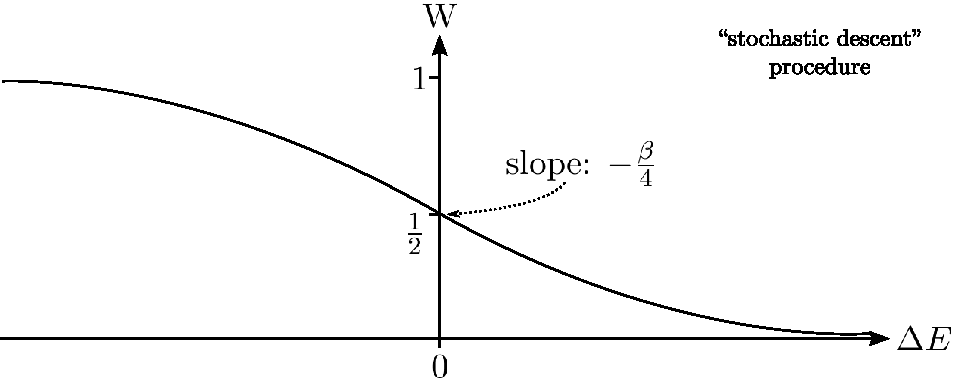
\includegraphics[width=8cm]{img/section3_fig1}
  \end{center}
  \begin{center}
  \vspace{-0.5cm}
  $\mathrm{W}_{(\vec{s}_t \rightarrow \vec{s})} = \frac{1}{1 + \exp( \beta_t \Delta E)}, \quad \Delta E = E_{(\vec{s})}- E_{(\vec{s}_t)}$\\
  \end{center}
\end{frame}

\notesonly{
The transition probability $\mathrm{W}$ measures the probability of changing to a new state $\vec s$ or remaining at $\vec s_t$. It depends on (A) the difference in cost and (B) the inverse temperature. The difference $\Delta E$ is the only way of measuring whether we gain any improvement from the transition or not. We use the inverse temperature $\beta_t$ to control how much we favor such transitions, or if we prefer a more conservative system. Below illustrates how the transition probability can be modulated by the inverse temperature $\beta$ during the annealing process:
}

\begin{frame} \frametitle{Modulating $\mathrm W$ during the annealing process}
%  \textbf{ limiting cases for high vs.\ low temperature:}
  \begin{center}
    \includegraphics[width=10cm]{img/switchfuns}
\vspace{5mm}
  \oident\oident\begin{tabular}[h]{c c c}
    low $\beta$ (high temperature) & intermediate $\beta$  & high $\beta$\\\\
    \includegraphics[width=3cm]{img/section3_fig4}
    & \hspace{-0.5cm}\includegraphics[width=3cm]{img/section3_fig5}
    & \includegraphics[width=3cm]{img/section3_fig6}
  \end{tabular}
\vspace{5mm}
  \end{center}
  \vspace{-2cm}
  \begin{tikzpicture}[scale=0.75]
\draw[->] (0,0) -- (1,0);
\draw[->] (0,0) -- (0,1.25);
% \draw[lightgray, very thick] (-1,0.5) -- (.9,0.5);
% \draw (0,0) node[anchor=north]{0};
\draw (0,1.25) node[anchor=west]{$E$};
\draw (1,0) node[anchor=west]{$\vec{s}$};
% \foreach \y in {0.5,1} \draw (0,\y) node[anchor=south east] {$\y$};
% \foreach \y in {0.5,1} \draw (-1pt,\y) -- (1pt,\y);
\end{tikzpicture}

\question{Which range of $\beta$ corresponds to \emph{exploration}/\emph{exploitation}?}\\

\end{frame}

\notesonly{
In the case of:

\begin{itemize}
\item low $\beta \corresponds$ high temperature:\\
The transition probability is nearly constant (W=0.5) regardless of $\Delta E$. It is equally probably to accept a transition or to remain at the same state. Therefore we can regard this as \emph{exploration} mode.
\item intermediate $\beta$:\\
Recall that we are currently considering a minimization problem. $\Delta E < 0$ whenever the new state is of lower cost than the previous one. We are no longer indifferent to this difference, but are more likely to accept transitions to lower-energy-states. Our process is still stochastic, therefore it is not guaranteed that we will accept every transition that yileds lower lower cost. We may either reject the transition and remain at the same higher-cost state or accept a transition to higher-cost state. such transitions are less likely to happen, but are still possible. This is where stochastic optimization is able to escape a local optimum and resume the search elsewhere instead of opting for the greedy approach. To reiterate, this is a stochastic process, if we sample long enough, we will find that intermediate values of $\beta$ are more likely to yield samples from the ``global'' minimum of this curve than the higher ``local'' minimum in this particular cost function.
\item high $\beta \corresponds$ low temperature:\\
This is the \emph{exploitation} mode. This reflects the behavior of a greedy learning algorithm such as gradient descent. Whenever we compare the cost of two successive states and find that $\Delta E < 0$ it tells us that the new state is of lower cost and more desirable for our minimization objective. The transition probability in this case will almost always accept a transition to a lower-cost state. Consequently it will almost always reject transitions to high-cost states, and the probability of remaining in a high-cost state is also very low. If the next sample is of lower-cost, we are very likely to accept that transition. Looking again at the stochastic nature of our process: We repeat the process multiple times and register how often each \emph{run} (not a single iteration) leads us to either minimum on this particular curve, we will find that the chances of finding the global minimum is just as likely as those of reaching the local minimum. This is because the initial state is the only decisive factor. high $\beta$ means we are in exploitation mode. We are only going to accept a transition if it lowers our cost. If we restrict our sampling to ``nearby'' states, we are emulating gradient descent. As soon as we've determined the direction of descent, we will follow it. The decisive factor is, where did we start? Since in our case, the two valleys around the two minima are equally ``wide'', it makes starting inside one equal to starting inside the other. If I am already in the vicinity of one minimum, the probability of transitioning \emph{outside} is very low. This probability is low, regardless of whether I am in the vicinity of the global or local minimum.
\end{itemize}
}

\begin{frame}\frametitle{Annealing schedule \& convergence}
Convergence to the global optimum is guaranteed if $\beta_t \sim \ln (t)$\footnote{shown in \citep{geman1984stochastic}}

\begin{itemize}
	% \itR robust optimization procedure
	\itR but: $\beta_t \sim \ln t$ is \textbf{too slow} for practical problems
	\itR therefore: $\beta_{t+1} = \tau \beta_t, \quad \tau \in [1.01,1.30]$
		(exponential annealing)
	\itR additionally: the \texttt{State Update loop} has to be iterated often enough, e.g. $M=500-2000$. \slidesonly{$\leadsto$ thermal equilibrium}
	\notesonly{This is required for reaching thermal equilibrium. Another way to look at it is the need to capture the stationary distribution of the states in relation to their cost. We will talk more about when we discuss the Gibbs distribution.}
\end{itemize}
\end{frame}

\subsection{The stationary distribution}

\begin{frame}


\slidesonly{
  \begin{center}
  \oident\oident\begin{tabular}[h]{c c c}
    low $\beta$ (high temperature) & intermediate $\beta$  & high $\beta$\\\\
    \includegraphics[width=3cm]{img/section3_fig4}
    & \hspace{-0.5cm}\includegraphics[width=3cm]{img/section3_fig5}
    & \includegraphics[width=3cm]{img/section3_fig6}
  \end{tabular}
\vspace{5mm}
  \end{center}
  \vspace{-2cm}
  \begin{tikzpicture}[scale=0.75]
\draw[->] (0,0) -- (1,0);
\draw[->] (0,0) -- (0,1.25);
% \draw[lightgray, very thick] (-1,0.5) -- (.9,0.5);
% \draw (0,0) node[anchor=north]{0};
\draw (0,1.25) node[anchor=west]{$E$};
\draw (1,0) node[anchor=west]{$\vec{s}$};
% \foreach \y in {0.5,1} \draw (0,\y) node[anchor=south east] {$\y$};
% \foreach \y in {0.5,1} \draw (-1pt,\y) -- (1pt,\y);
\end{tikzpicture}

Missing a probability distribution across states.
}

\notesonly{
As we discussed the effect of $\beta$ on the transition probability, we saw how this controls explorations and exploitation. 
By talking about the probability of descending vs. jumping to a completely different location, we also talked about the probability of landing inside the valley surrounding the global minimum vs. that surrounding a \emph{local} one. Therefore, it becomes necessary to define a measure for the probability for each possible state that $\vec s$ can take. 
This measure needs to fulfill the following requirements: 
\begin{enumerate}
\item Reflect the probability distribution across states
\item For constant $\beta$ it should converge to the stationary distribution. That is the probability of transitioning from some state $\vec s$ to $\vec s'$ should be equal to the reverse transition. This is what is meant by ``thermal equilibrium''.
\end{enumerate}
}
\end{frame}

\subsection{Calculation of the stationary distribution}

\begin{frame}{\subsecname}

\svspace{-5mm}

%\question{How do we find this stationary distribution?}

%\pause

%\vspace{-0.5cm}
\begin{equation}
	\underbrace{ \substack{	\text{probability of} \\
				\text{transition } 
				\vec{s} \rightarrow \vec{s}^{'}} }_{
			P_{(\vec{s})} \mathrm{W}_{(\vec{s} \rightarrow
				\vec{s}^{'})} }
	 = 
	\underbrace{ \substack{	\text{probability of} \\
				\text{transition } 
				\vec{s}^{'} \rightarrow \vec{s} } }_{
			P_{(\vec{s}^{'})} 
			{\color{blue}
			\mathrm{W}_{(\vec{s}^{'} \rightarrow
				\vec{s})}} }
\end{equation}
%\begin{equation*}
	%\begin{array}{ll}
	%\frac{P_{(\vec{s})}}{P_{(\vec{s}^{'})}}
	%& = \frac{\mathrm{W}_{(\vec{s}^{'} \rightarrow \vec{s})}}{
		%\mathrm{W}_{(\vec{s} \rightarrow \vec{s}^{'})}} 
	%= \frac{1 + \exp\big\{ \beta \big( E_{(\vec{s})} - E_{(\vec{s}^{'})}
		%\big) \big\} }{1 + \exp\big\{ \beta \big( E_{(\vec{s}^{'})} - 
		%E_{(\vec{s})}\big) \big\} }
	%= \frac{1 + \exp( \beta \Delta E)}{1 + \exp( -\beta \Delta E)}  \\\\
	%\pause
	%& = \exp( \beta \Delta E) \frac{1 + \exp( -\beta \Delta E)}{
		%1 + \exp( -\beta \Delta E) } 
	%= \exp( \beta \Delta E ) \\\\
	%\pause
	%& = \exp\big\{  \beta \big( E_{(\vec{s})} - E_{(\vec{s}^{'})}\big) \big\}
	%= \exp\big\{ \beta E_{(\vec{s})} -  \beta E_{(\vec{s}^{'})} \big\}\\\\
	%&= \frac{\exp\left( \beta E_{(\vec{s})}\right)}{\exp\left( \beta  E_{(\vec{s}^{'})} \right)}
    %\slidesonly{
    %\qquad \small \text{condition is fulfilled by Gibbs distribution.}
    %}
	%\end{array}
%\end{equation*}
\begin{align}
	\frac{P_{(\vec{s})}}{P_{(\vec{s}^{'})}}
	& = \frac{{\color{blue}\mathrm{W}_{(\vec{s}^{'} \rightarrow \vec{s})}}}{
		\mathrm{W}_{(\vec{s} \rightarrow \vec{s}^{'})}} 
	= \frac{1 + \exp\big\{ \beta \big( E_{(\vec{s}^{'})} - E_{(\vec{s})}
		\big) \big\} }{{\color{blue}1 + \exp\big\{ \beta \big( E_{(\vec{s})} - 
		E_{(\vec{s}^{'})}\big) \big\} } }
	= \frac{1 + \exp( -\beta \Delta E)}{{\color{blue}1 + \exp( \beta \Delta E)}}  \\
	&= {\color{blue}\frac{1}{1+\exp(\beta \Delta E)}} \exp(-\beta \Delta E)
	\Big\lbrack \exp(\beta \Delta E) + 1\Big\rbrack\\
	&= \exp(-\beta \Delta E) \frac{1+\exp(\beta \Delta E)}{{\color{blue}1+\exp(\beta \Delta E)}}
	= \exp( - \beta \Delta E ) \\
	& = \exp\big\{ -\beta \big( E_{(\vec{s})} - E_{(\vec{s}^{'})}\big) \big\}\\
	%= \exp\big\{ \beta E_{(\vec{s}^{'})} -  \beta E_{(\vec{s})} \big\}\\
	&= \frac{\exp\left( -\beta E_{(\vec{s})}\right)}{\exp\left( -\beta  E_{(\vec{s}^{'})} \right)}
    \slidesonly{
    \qquad \small \text{condition is fulfilled by Gibbs distribution.}
    }
\end{align}
\notesonly{
The condition is fulfilled for the \emph{Gibbs-Boltzmann} distribution:
}

\end{frame}
\begin{frame}\frametitle{The Gibbs distribution}
\notesonly{
The Gibbs (or Boltzmann-) distribution from statistical physics, measures the
probability of a system to be in state $\vec s$ having Energy $E_{(\vec s)}$ is
given as
}
\begin{equation}  \label{eq:gibbs}
P_{(\vec{s})} := \frac{1}{Z} \exp \Big(-\frac{E_{(\vec s)}}{k_b T}\Big) 
= \frac{1}{Z} \exp \Big(-\beta E_{(\vec s)} \Big) 
\end{equation}

where the normalization constant / partition function $Z$ is defined as:


\begin{equation} \label{eq:partition}
Z := \sum\limits_{\vec{s}} \exp \Big(-\frac{E_{(\vec s)}}{k_b T}\Big) = \sum\limits_{\vec{s}} \exp(-\beta E_{(\vec s)})
\end{equation}

\notesonly{
The partition function $Z$ ensures that $P_{(\vec{s})}$ is a probability
measure and the Boltzmann constant $k_b = 1.38 \cdot 10^{-23} J/K$
gives a scale of the \emph{temperature} $T$. This means the
probability of observing a state is fully determined by its Energy.

%For sampling algorithms one often constructs a Markov chain whose
%stationary distribution is a Gibbs-distribution for a specified cost
%(or energy-) function.
}

\end{frame}

\begin{frame}\frametitle{Cost vs. probability distribution}
\question{How does $\beta$ modulate $P_{(\vec s)}$?}

$E_{(\vec{s})}$
\vspace{-0.2cm}
\begin{figure}[h]
  \centering
\includegraphics[width=12cm]{img/section3_fig7}  
\[ \begin{array}{ll}
	\beta \downarrow:\pause
	& \text{broad, ``delocalized'' distribution} \\\vspace{-0.3cm}\\
	\beta \uparrow:\pause
	& \text{distribution localized around (global) minima}
\end{array} \]
\end{figure}


\end{frame}

%\newpage

\notesonly{
We will now further formalize what is going on with simulated annealing.
}

\mode*

%\mode<all>
%\section{Monte Carlo Markov Chain (MCMC)}


\begin{frame}



Whenever it is difficult to evaluate the joint distribution\\
opt for ``learning through trial and error''\\

\notesonly{
MCMC methods are a popular
strategy in situations where it is hard to evaluate the joint (e.g.\
posterior distribution) of a rnadom variable analytically but where it is easy to
sample from the conditional distribution (and finally the joint
distribution). Using samples from such a posterior distribution, one
can estimate many summaries of interest without explicitly knowing the
joint distribution\footnote{credit to Dr. Timm Lochmann for the content on MCMC}.

}

\slidesonly{
\vspace{1cm}
What is:

\begin{itemize}
\item a Markov Chain
\item the Markov property
\item the stationary distribution
\item Monte Carlo
\item the Metropolis algorithm
\item Metropolis sampling (Monte Carlo + Markov Chain) - simulated annealing
\item deterministic annealing (variational approach) - for further reading
\end{itemize}

The following is for providing a framework around stochastic optimization.
}

\end{frame}
\begin{frame} \frametitle{Markov chain and the Markov property}
Consider a family of random variables $X_t$, $t=1,2,\ldots$, which describe a stochastic process. $x_t$ denotes the state at time $t$.

\notesonly{
A sequence of such is referred to as a \emph{Markov chain} whenever $X_{t+1}$ depends only on the predecessor $X_t$ and is \emph{independent} of all values previous to that:
}

\begin{align}
\label{eq:markovprop}
P(X_{t+1} &= x_{t+1} | X_{t} = x_{t}, X_{t-1} = x_{t-1}, \ldots, X_{0} = x_{0})\\
&= P(X_{t+1} = x_{t+1} | X_{t} = x_{t})
\end{align}

\notesonly{\eqref{eq:markovprop}}
\slidesonly{This} is refered to as the \emph{Markov property}. 
\notesonly{The conditional distribution of $X_t$ depends only on its
predecessor. In the more general case of Markov Random Fields, the
Markov property induces a ``local neigborhood''/ set of \emph{parents}
which fully determines the conditional distribution).}
The transition probabilities between subsequent states
$$
P(X_{t+1}=j|X_{t}=i)=p_{ij}
$$
can be described via the stochastic matrix $M = \{m_{ij}\}_{ij}$ with
$m_{ij}=p_{ij}$. 
\\

\pause

\slidesonly{Exactly what $W$ in simulated annealing describes for the states $\vec s$:
}
\notesonly{
The transition probability $W$ we just encountered in simulated annealing with states $\vec s$ describes exactly this:
}
\begin{align}
\label{eq:markovproptransition}
W_{s_i \rightarrow s_j} = P(X_{t+1} = s_j | X_{t} = s_i)
\end{align}

\begin{center}
s.t. $W_{s_i \rightarrow s_j} > 0 \;\;\forall (i,j)\quad$
and $\quad\sum_j W_{s_i \rightarrow s_j} = 1 \;\;\forall i$.

\end{center}
\end{frame}

\begin{frame}\frametitle{Stationary distribution:}
\label{sec:stat-distr}
The \emph{stationary distribution} of a homogeneous Markov chain is a
distribution $\pi=[\pi_1,\pi_2,..., \pi_N$] such that
\begin{equation}
M \pi  = \pi
\end{equation}
where 
\begin{align}
p(x_{t+1}=j) &= \sum_i p(x_{t+1}=j,x_{t}=i) \\
&= \sum_i p(x_{t+1}=j|x_{t}=i)\,p(x_{t}=i)\\
&= M \pi
\end{align}
and can be derived from the eigen-decomposition of the transition matrix
(given certain conditions on the Markov chain $\rightarrow$ irreducibility, recurrence etc.)

If the Markov chain is \emph{reversible}, the stationary distribution is
characterized by a \emph{detailed balance} between going from one
state to another one, i.e.\
$$
\pi_i p_{ij} = \pi_j p_{ji}
$$
\end{frame}

\begin{frame}\frametitle{Monte Carlo}
\notesonly{
Monte Carlo methods
have been used to } evaluate certain integrals with stochastic methods.\\

Example:\\
Estimate $\pi$ via random sampling from $[0,1]$ and counting how
many of the points have distance smaller than 1. Using the fact that
$A = \pi r^2$ and $4 A/F_\mathrm{square} = 4 N_\mathrm{A}/N$ gives $\approx \pi$.
\\
\end{frame}

\begin{frame}
\slidesonly{
\frametitle{Monte Carlo}
Evaluating probability of states (e.g.\ to compute integrals, expectation values
etc.) is difficult.
Easier to sample from conditional distributions.\\

Approaches:
\begin{enumerate}
\item Gibbs sampler:\\
    Sample from conditional distribution to produce a Markov chain with the joint
posterior density as its stationary distribution.
\item Metropolis algorithm:\\
    sampling strategy with which to accept or reject transitions
\end{enumerate}
}
\end{frame}

While it can be difficult to evaluate the
probability of states (e.g.\ to compute integrals, expectation values
etc.) it is possible to sample from the joint distribution by
sequential sampling from conditional distributions that are easier to
compute. There are two approaches: the \emph{Gibbs sampler} and
\emph{Metropolis} type algorithms (Note: this material is taken nearly
verbatim from Kass et. al. 1997, roundtable discussion??).

\subsection{Gibbs sampler:}
\label{sec:gibbs-sampler}

The Gibbs sampler \citep{GemanGeman1984} samples from the collection
of full (or complete) conditional distributions and it does, under
fairly broad conditions, produce a Markov chain with the joint
posterior density as its stationary distribution.  A tutorial can be
found in \citep{CasellaGeorge1992}.

\newpage
\begin{frame}\frametitle{Metropolis algorithm}

\notesonly{
When it is difficult to directly sample from the conditionals, one may
instead simulate from a different Markov chain with a different
stationary distribution, but then modify it in such a way so that a
new Markov chain is constructed which has the targeted posterior as its
stationary distribution. This is done by the Metropolis-Hastings
algorithm -- It samples from a prespecified candidate (proposal)
distribution for and subsequently uses an accept-reject step (see Kass
et. al. 1997).
}

The \emph{Metropolis algorithm} describes the sampling strategy with which to accept or reject transitions:
\begin{equation}
P(Y_n = x_j | X_{n} = x_i) = P(Y_n = x_i | X_{n} = x_j)
\end{equation}

IF $\Delta E < 0$ (minimization) then \\

\oident accept transition \\

ELSE \\

\oident Sample $\varepsilon$ from $\mathcal{U} \sim \lbrack 0, 1 \rbrack$ \\

IF $\varepsilon < \exp \left( - \beta \Delta E \right)$ then \\

\oident accept transition

\oident the new state is similar/``close'' to the prev. state (e.g. bit flip)\\


ELSE\\

\oident reject transiton and remain at the same state\\

\vspace{0.5cm}
Simulated annealing follows the Metropolis algorithm.

\end{frame}

\begin{frame}\frametitle{Metropolis sampling}
\label{sec:metropolis-sampling}
The MCMC strategy of Metropolis sampling uses a 2-step approach
\begin{enumerate}
\item Markov Chain $\rightarrow$   Proposal Density
\item Monte Carlo $\rightarrow$   Acceptance Probability
\end{enumerate}

\textbf{Proposal Distribution:}
The Proposal density determines which nodes to \emph{poll} (``select
and test'') next and needs to fulfil the following properties:
\begin{itemize}
\item nonnegative: $\tau_{ij} \geq 0$ 
\item normalized: $\sum_j \tau_{ij} =1$ 
\item symmetric: $\tau_{ij}=\tau_{ji}$
\end{itemize}

\end{frame}

\newpage

\subsection{Acceptance Probability:}
This probability specifies how likeli it is to go from state $i$ to
$j$. In our scenario, this depends only on their energy levels (and the current value of
temperature).

\subsection{Example:} Using the difference in energy levels 
$\Delta_{ij} = E_j -E_i$, the sigmoidal acceptance rule is given as
$$
p_\mathrm{switch}(i \rightarrow j) = p_{ij} = \frac{1}{1+e^{\Delta_{ij}}} = \frac{1}{1+e^{(E_j -E_i)}}.
$$
From the assumption of detailed balance then follows
\begin{eqnarray*}
  \tau_i p_{ij} & = & \tau_j p_{ji}\\
  \frac{\tau_i}{\tau_j}& = &  \frac{p_{ji}}{ p_{ij}} 
= \frac{1+\exp(\Delta_{ij})}{1+\exp(\Delta_{ji})}
= \frac{1+\exp(\Delta_{ij})}{1+\exp(-\Delta_{ij})}\\
& = & \exp(\Delta_{ij}) \frac{1+\exp(\Delta_{ij})}{1+\exp(\Delta_{ij})}
= \exp(\Delta_{ij})\\
&= &\exp(E_j-E_i) = \frac{Z \exp(E_i)}{Z \exp(E_j)}
\end{eqnarray*}
demonstrating that 
$p(X_i)= \frac{1}{Z} \exp \big(-\frac{E_i}{k_b T}\big)$
is a consistent choice. 
\\

\begin{itemize}
\item Determination of the \emph{transition probability} $p(X_T|X_{j})$
  requires only knowledge of $E_i - E_j$. Applying the Metropolis
  algorithm with these parameters will lead to a stationary
  distribution $\pi$ with $\pi_i= p(x_i)$.
\item This means, we can sample from the distribution $p_\beta(x)$
  without knowing $Z=\sum_{i \in I} \exp(-\beta E_i)$ which is
  difficult to estimate for large $I$ as e.g.\ $2^N$.
\item Acceptance depends only on the \emph{energy difference} between
  the current and suggested state. This difference depends only on the
  \emph{neighborhood} of the polled unit an not necessarily the full
  system!
\end{itemize}

\question{How does this all tie back to Simulated Annealing?}

Making use of the temperature parameter (and an annealing schedule),
Metropolis sampling can be used to optimize cost functions.

\textbf{Motivation:} At each temperature, the MCMC relaxes into the
stationary distribution. For lower and lower temperatures (higher $\beta$), the entropy
of this distribution becomes lower and lower, more ``peaked'', i.e.\
only the \emph{most} probable states have nonzero probability. 
The probability of states that initial started with moderate or lower probability values are pulled towards near-zero values. 
\textbf{Also}: The average
Energy becomes lower and lower. This motivates simulated annealing as
an optimization approach.

\begin{itemize}
\item For each temperature, relax towards stationary distribution
\item gradually decrease temperature
\item[$\leadsto$] observed states represent approximately ``optimal solutions''
\end{itemize}
If the shape of distribution changes smoothly and cooling is ``slow
enough'', this will result in a distribution concentrated on the
minimum-energy state, i.e. will end up in an optimal solution with
probability 1.

\subsection{Simulated (stochastic) annealing (revisited)} \label{sec:stochastic-annealing}
``classical'' MCMC approach: select variable, stochastically accept
change in state for that variable. 

Depending on the distribution, sampling might be the only feasible
solution.  There are different strategies (Gibbs sampling,
Proposal-Reject) depending on whether direct sampling from the
conditional distributions makes Gibbs-Sampling possible.


\textbf{Caveat:} Sampling takes a lot of time and depends on the
annealing schedule. In some cases, deterministic strategies can make
use of efficient approximations of the true distribution and thereby
significantly speed up the optimization proces.




%\mode*

\clearpage

\mode<all>
\section{Mean-field (deterministic) annealing} \label{sec:mean-determ-anne}

\mode<presentation>{
\begin{frame} 
    \begin{center} \huge
        \secname
    \end{center}
    \begin{center}
    Take simulated annealing \\
    but \\
		go faster, go deterministic
    \end{center}
\end{frame}
}

\begin{frame}{\secname}
 %\vspace{-2mm}
%\begin{block}{Simulated Annealing}
%\begin{itemize}
%\itr stochastic optimization: computationally expensive (sampling!)
%\itr stationary distribution $P_{(\vec{s})}$ known (for each $\beta_t$), why not evaluate?
%\itr but: maxima of $P_{(\vec{s})}$ equally hard to obtain as minima of $E_{(\vec{s})}$
%\itr moments? for $\beta \rightarrow \infty$: $\langle \vec{s} \rangle_P$ converges to $\vec{s}^*$ of minimal cost (caveat: true only if $P_{(\vec{s})}$ has only one global optimum)
%\itr but: moments of $P_{(\vec{s})}$ can -- in general -- not be calculated analytically
%\end{itemize}
%\end{block}
%\vspace{-2mm}
\slidesonly{
\begin{center}
\includegraphics[width=12cm]{img/section3_fig7}  
\end{center}
}

\only<1>{

\begin{block}{Approximation by Mean-Field Annealing}
\begin{itemize}
\itR idea: approximate $P_{(\vec{s})}$ by a computationally tractable distribution $Q_{(\vec{s})}$
\itR this distribution is then used to calculate the first moment $\langle \vec{s} \rangle_Q$\\
\itR the first moment is tracked during the annealing schedule $\beta_t$
\itR hope: $\displaystyle \langle \vec{s} \rangle_Q \to $ $\vec{s}^*$ for $\beta_t\to\infty$
\end{itemize}
\end{block}

}

\only<2>{
\question{Why fixate on the first moment?}

\pause

- to localize the peak of the distribution as entropy decreases. 
At $\beta_t \rightarrow \infty$, the peak will have localized around the state where the cost is minimal, revealing the optimal state $\vec s^*$

}

\only<3>{

\question{Do we still need the annealing process?}

-Yes, because still need a tradeoff between exploration and exploitation.
}

 
\end{frame}

\subsection{Factorizing distribution}

\begin{frame}{\subsecname}
\begin{block}{Distribution $Q_{(\vec{s})}$ to approximate $P_{(\vec{s})}$}
\vspace{-0.35cm}
\begin{equation}
	Q_{(\vec{s})} \quad
= \quad \frac{1}{Z_Q} \exp \left\{ -\beta E_Q\right\} \quad
= \quad \frac{1}{Z_Q} \exp \Big\{ -\beta \sum\limits_{k}
		\underbrace{ e_k }_{ \text{parameters} } \mathrm{s}_k \Big\}
\end{equation}
\vspace{-0.65cm}
\begin{itemize}
 \item Gibbs distribution with costs $E_Q$ linear in the state variable $\vec{s}_k$
 \item factorizing distribution $Q_{(\vec{s})} = \Pi_k Q_k(s_k)$ with $Q_k(s_k) 
 = \frac{1}{Z_{Q_k}} \exp (-\beta e_k\mathrm{s}_k)$
% \end{itemize}
% \end{block}
% \vspace{-0.2cm}
% \begin{block}{Properties of $Q$}
% \begin{itemize}
 \item $Q_{(\vec{s})}$ factorizing $\iff s_k$ independent $\implies
    \langle \Pi_k s_k \rangle_Q = \Pi_k \langle s_k\rangle_Q
    \quad \!\! (\substack{\text{moments}  \\ \text{factorize}})$
 \item
 $ \big< s_k \big>_Q = \frac{\sum\limits_{s_k} s_k \exp(-\beta e_k s_k)}{
					\sum\limits_{s_k} \exp(-\beta e_k s_k)}$
\end{itemize}
\end{block}
% \vspace{-0.3cm}
\begin{itemize}
      \itr family of distributions parametrized by the \emph{mean fields} $e_k$
      \itr determine $e_k$ such that this approximation is as good as possible
\end{itemize}
\end{frame}


\begin{frame}{Mean-field approximation}
\begin{block}{Quantities}
\begin{equation}
	\begin{array}{llc}
	P_{(\vec{s})} 
	& = \frac{1}{Z_p} \exp(-\beta E_p) 
	& \substack{ \text{true distribution} } \\
	Q_{(\vec{s})} 
	& = \frac{1}{Z_Q} \exp\big(-\beta \overbrace{\sum\limits_k e_k s_k}^{E_Q} \big)
	& \substack{ \text{approximation: family of} \\ \text{factorizing distributions} } \\\\
	e_k:
	& \text{\textit{mean fields} }
	& \substack{ \text{parameters to} \\ \text{be determined} }
	\end{array}
\end{equation}
\end{block}
\begin{block}{Good approximation of $P$ by $Q$}
\vspace{0.1cm}
$\rightarrow$ minimization of the KL-divergence:
\begin{equation}
	\dkl(Q||P) = \sum\limits_{\vec{s}} Q_{(\vec{s})} \ln \frac{Q_{(\vec{s})}}{
		P_{(\vec{s})}} \eqexcl \min_{\vec{e}}
\end{equation}
\end{block}
\end{frame}

\subsubsection{Setting up the arguments for the KL divergence}

\begin{frame}{\subsubsecname}

Let $P$ be the reference distribution (target) and $Q$ be the parameterized distribution (what we tune).

\question{How do we generally decide between minimizing $\dkl(Q||P)$ vs. $\dkl(P||Q)$?}

\pause

-We look at what kind of solutions are found by each usage of the KL divergence:  


\end{frame}

\begin{frame}{\subsubsecname}

\begin{block}{minimizing forward $\dkl$}

\slidesonly{
\begingroup
\footnotesize
}
\begin{equation}
	\dkl(P||Q) = \sum\limits_{\vec{s}} P_{(\vec{s})} \ln \frac{P_{(\vec{s})}}{
		Q_{(\vec{s})}} \eqexcl \min_{\text{parameters}}
\end{equation}
\slidesonly{
\endgroup
}
\end{block}

\begin{itemize}
\item \notesonly{Corresponds to }the \emph{maximum-likelihood} solution\notesonly{ (will discuss later in density estimation)}
\item Seen in Infomax and density estimation.
\item Change $Q$ such that it ``covers'' as much of $P$ as possible.
\notesonly{\item If $P$ has two modes minimizing $\dkl(P||Q)$ will find a $Q$ that is wide enough to cover both.}
\end{itemize}

\pause

\begin{center}
	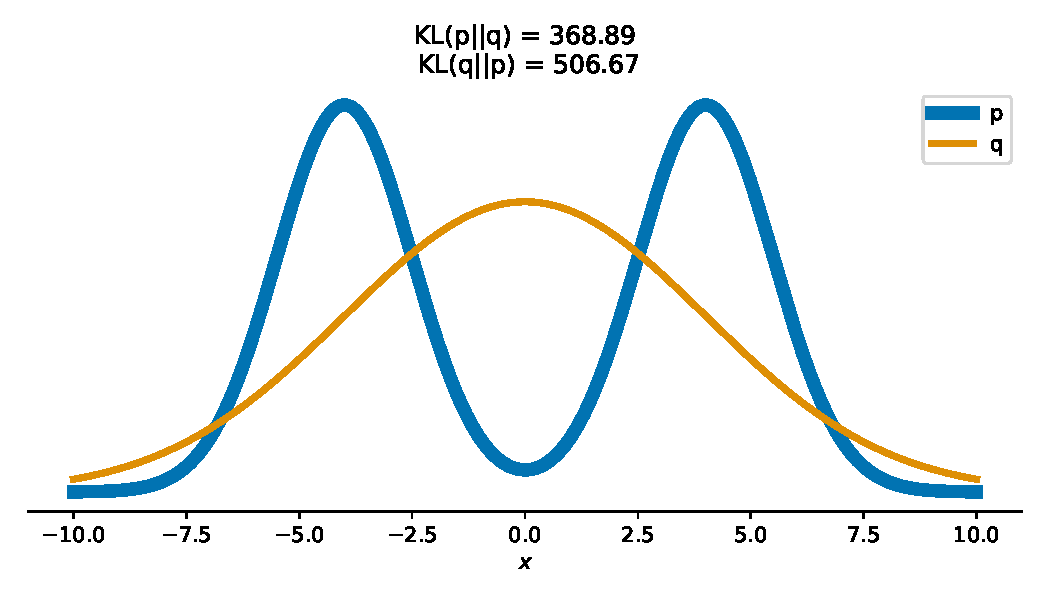
\includegraphics[width=0.55\textwidth]{img/kl_fwd}
\end{center}

\end{frame}

\begin{frame}{\subsubsecname}

\begin{block}{Reverse $\dkl$}
\slidesonly{
\begingroup
\footnotesize
}
\begin{equation}
	\dkl(Q||P) = \sum\limits_{\vec{s}} Q_{(\vec{s})} \ln \frac{Q_{(\vec{s})}}{
		P_{(\vec{s})}} \eqexcl \min_{\text{parameters}}
\end{equation}
\slidesonly{
\endgroup
}
\end{block}

\begin{itemize}
\item Corresponds to the \emph{maximum-entropy} solution.
\item With $Q$ in the numerator of the $\log$ we prefer solutions where $Q$ is zero even if $P$ is non-zero. 
\end{itemize}

\pause
\only<2>{
\slidesonly{
\begin{center}
	
\includegraphics[width=0.3\textwidth]{img/meme_revkl}
\end{center}

}
}

\only<3>{

\begin{center}
	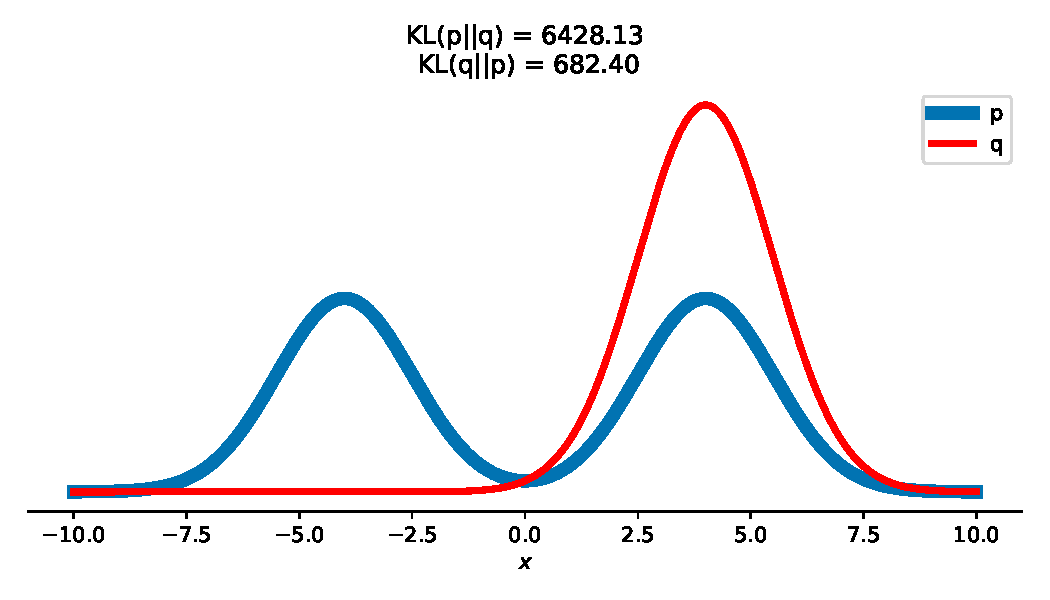
\includegraphics[width=0.55\textwidth]{img/kl_rev}
\end{center}

\notesonly{If $P$ has two modes a ``good'' $Q$ is one that fits one mode very well even if it completely ignores the other mode\footnote{Additional resources for explaining the differences between forward and reverse KL:\\ 
\href{https://dibyaghosh.com/blog/probability/kldivergence.html} \\ and \\
%\href{https://www.quora.com/What-is-the-theoretical-advantage-disadvantage-between-minimizing-KL-Q-P-and-KL-P-Q-in-Bayesian-variational-inference}
}.
}
}
\end{frame}

\begin{frame}

\question{Why minimize the reverse $\dkl$ for mean-field approximation?}

\slidesonly{
\begin{equation}
	\dkl(Q||P) = \sum\limits_{\vec{s}} Q_{(\vec{s})} \ln \frac{Q_{(\vec{s})}}{
		P_{(\vec{s})}} \eqexcl \min_{\vec{e}}
\end{equation}
}

- Even if our assumption about $P$ having a single moment is wrong. If it has two minima, picking one is better than picking a solution in the middle.

\end{frame}

\subsubsection{Mean-Field annealing for Ising model}

\begin{frame}{Mean-field annealing\only<2>{~ for Ising model}}
\begin{block}{Algorithm}
% \begin{algorithm}[h]
%   \DontPrintSemicolon
%   initialization: $\langle \vec{s} \rangle_0, \beta_0, t = 0$ \;
%   \Begin(Annealing loop){ 
%     \Repeat{$|e_k^\mathrm{old}-e_k^\mathrm{new}| < \varepsilon$}
%     {
%       calculate mean-fields: $e_k, \ \ k = 1, \ldots, N$ \;
%       calculate moments: $\big<s_k\big>_Q,\ \ k = 1, \ldots, N$ \;
%     }
%     increase $\beta$ \;
%     }
%   \end{algorithm}
% 

\texttt{initialization:} $\langle \vec{s} \rangle_0, \beta_0$ \; \\
\texttt{BEGIN Annealing loop}\\
\oident \texttt{Repeat} \\
\begin{itemize}
  \item calculate mean-fields: $e_k\visible<2>{= - \sum\limits_{\substack{i=1 \\ i\ne k}}^N W_{ik} \langle s_i \rangle_Q}, \ \ k = 1, \ldots, N$ \;
  \item calculate moments: $\big<s_k\big>_Q\visible<2>{= \tanh(-\beta e_k)},\ \ k = 1, \ldots, N$ \;
\end{itemize}
\oident\texttt{Until $|e_k^\mathrm{old}-e_k^\mathrm{new}| < \varepsilon$} \\
\oident increase $\beta$ \; \\
\texttt{END Annealing loop}
\end{block}
\end{frame}

\begin{frame}
\slidesonly{
\begin{center}
\includegraphics[width=12cm]{img/section3_fig7}  
\end{center}
}
\end{frame}

%\section{Deterministic annealing} \label{sec:determ-anne}

\begin{frame}

Mean field methods provide a specific type of variational approach for
optimization problems (\cite{Bishop2006,Murphy2012}). This is useful
more generally for density estimation ($\rightarrow$ Variational
Bayes) where it often provides a more efficient option than sampling
techniques if the posterior distribution can be well approximated by a
factorizing distribution. The following description of the variational
approach closely follows \citep[ch. 21.3]{Murphy2012}.

\textbf{more about this in the notes.}\\
\textbf{switch to mean field lecture slides}

\end{frame}

\begin{eqnarray*}
  \label{eq:1}
 L(q_i) & = & \sum_x \prod_i q_i(x_i) \Big( \log \tilde{p}(x) - \sum_k \log q_k(x_k) \Big) \\
 & = & \sum_{x_j} \sum_{x_{-j}} q_j (x_j) \prod_{i \neq j} q_i(x_i) \Big( \log \tilde{p}(x) - \sum_k \log q_k(x_k)   \Big) \\ 
 & = & \sum_{x_j} q_j(x_j) \sum_{x_{-j}} \prod_{i \neq j} q_i(x_i) \log \tilde{p}(x) \\
& &  - \sum_{x_j} q_j(x_j) \sum_{x_{-j}} \prod_{i \neq j} q_i(x_i) \Big(\log q_j(x_j)+ \sum_{k \neq j} \log q_k(x_k) \Big) \\ 
& = &  \sum_{x_j} q_j(x_j) \log f_j(x_j) - \sum_{x_j} q_j(x_j) \log q_j(x_j) +  const
\end{eqnarray*}
where we introduced the definition
$$
\log f_j(x_j):= \sum_{x_{-j}} \prod_{i \neq j} q_i(x_i) \log
\tilde{p}(x). 
$$
Although $f_j$ is not a proper distribution (not normalized), the last
term can be interpreted as a KL-divergence
$$
L(q_j) \sim - \dkl(q_j||f_j).
$$
Therefore, $L(q) = - \dkl(q||\tilde{p})$ can be maximised by
minimizing $\dkl(q_j||f_j)$  i.e. setting $q_j = f_j$ by
$$
q_j(x_j) = \frac{1}{Z_j} \exp\big(\E_{-q_j}[\log \tilde{p}(x)]\big)
$$
Ignoring the normalisation constant we get as the optimal component $q_j$
\begin{equation}
  \label{eq:MeanField}
\log q_j(x_j) = \E_{-q_j}[\log \tilde{p}(x)]  
\end{equation}

\subsection{Alternative motivation of the mean-field annealing
  approach} \label{sec:motivation} at each step we actually know
$p_{\Delta E}(\mathrm{flip})$ which enables us to estimate
$E[X_i|X_{-i}]$ i.e.\ the average value of $X_i$ given its parents.

Mean field annealing generalizes this approach by making use of the fact that 
the marginal distributions of $X_i$ are known in this way and then using the relation: 
i.e.\ with $p(v_j) = \frac{1}{1+e^{-v_j/t}}$ we can write: 
$$
\langle x_j \rangle =  (+1) P(v_j) +(-1)(1-P(v_j)) = 2 P(v_j) -1 = \tanh(v_j/2T)
$$
Although v is not known exactly (depends on the exact states of the
other $X$ and their interactions) we can approximate it as
$$
v_j \approx \langle v_j \rangle = \Big\langle \sum_i w_{ji} x_i \Big\rangle = 
 \sum_i w_{ji}  \langle x_i \rangle 
$$
where $\langle v_j \rangle$ is called the ``mean field'' and gives the average value of $x_j$ as 
$$\langle x_j \rangle \approx \tanh\frac{\langle v_j\rangle}{2T}$$

\textbf{Relation between the sigmoidal and tanh:} Using the sigmoidal acceptance probability is equivalent to using $\tanh$ for \emph{states} $x \in \{-1,+1\}$  of the RV i.e.\ $\tanh(z) \in (-1,1)$ for $z \in (-\infty,+\infty)$. 

\begin{equation}
\tanh(x) = \quad\frac{e^{2x}-1}{e^{2x}+1} 
 \quad = \frac{1-e^{-2x}}{1+e^{-2x}} \quad = \frac{2-1-e^{-2x}}{e^{-2x}+1} \quad =  \frac{2}{1+e^{-2x}} -1 
\end{equation}
or the other way round: 
$$
\frac{1}{1+e^{-x}} = \frac{1}{2}\left(1+\tanh(\frac{1}{2}x)\right)
$$

\section{Boltzmann machines}
\label{sec:boltzmann-machines}

Approach can be generalized to hidden units and details on Boltzmann
machines in \cite{AartsKorst1990}. Restricted BMs (RBMs) do not have connections between observable or hidden units, which simplifies computation of conditional probabilities necessary for learning considerably. RBMs have been developed (among others) by P. Smolensky, who called them "Harmoniums" (\cite{Smolensky1986}). 
\begin{itemize}
\item General model of distributions
\item parameters (W) can be learned from samples
\item works for Systems with nonobservable (latent) variables 
\item interesting model of cognitive processes
\item structured boltzmann machines as efficient pattern recognition systems
\end{itemize}


\mode*

\clearpage

\section{References}
\begin{frame}[allowframebreaks] \frametitle{References}
	\scriptsize
	\bibliographystyle{plainnat}
	\bibliography{bibliography}
\end{frame}

\end{rightcolumn}
\end{paracol}

\end{document}
